
\section{Obstacle avoidance}
\begin{marginfigure}
	\centering
	%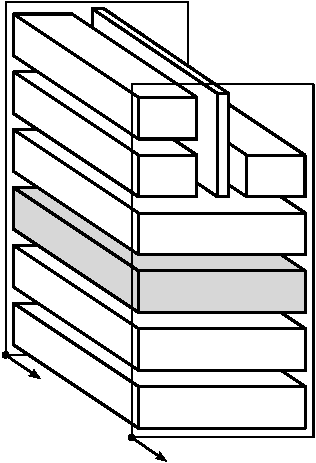
\includegraphics[scale=0.5]{ch3/img/PA_map_obstacle.pdf}
	\begin{tikzpicture}[>=latex',scale=0.4]
	\drawplanexy{-0.3}{-0.3}{-0.3}{6.7}{10}{dashed}{perception}
	
	\drawcube{0}{0}{5}{6.4}{1}{white}{dinamica}{}{};
	\drawcube{0}{1.2}{5}{6.4}{1}{white}{tracking}{}{};
	
	\drawcube{0}{2.4}{5}{6.4}{1}{gray!40}{ostacoli}{}{};
	\drawcube{0}{3.6}{5}{6.4}{1}{white}{altitude}{}{};
	
	\drawcube{0}{4.8}{5}{3}{1.5}{white}{source}{}{};
	\drawcube{0}{6.5}{5}{3}{1.5}{white}{emulatore}{}{};

	\drawplanezy{3.2}{4.8}{5}{4.5}{radar_det}{fill=white,opacity=0.90}{}{};

	\drawcube{3.4}{4.8}{5}{3}{3.2}{white}{alpha}{}{};
	\drawplanexy{-0.3}{-0.3}{5.3}{6.7}{10}{dashed}{action}
	

	\draw [->,line width=1.5] (action_D) -- ++(0,0,2);
	\draw [->,line width=1.5] (perception_D) -- ++(0,0,2);

	\coordinate [at=(radar_det_D), yshift=-5] (arrows_point);
	\draw [->,dashed]  (arrows_point) -- ++(1.5,0,0); 
	\draw [->,dashed]  (arrows_point) -- ++(-1.5,0,0); 
\end{tikzpicture}
\end{marginfigure}
An avalanche has an huge amount of kinetic energy, enough to destroy most of the artificial building and move objects with a big cross--section that are on its traveling path. Thus, the objects that avalanche drone has to avoid are mainly pillars, trees or mounds of snow.

Taken into account this consideration about the surroundings in which the drone will try to find a buried person, it is useless to define an internal map of obstacle and elaborate the optimal trajectory to an ending point because, in fact, for the most of the time the drone will explore without having such a knowledge of the ending point.

This simplification gather different advantage to the final algorithm:
\begin{itemize}
\item we do not need the extremely high computational power needed to maintain such environment projection into agent mind space
\item the obstacle avoidance imposes minor constraints on the upper layer of the searching algorithm, with respect to convoluted algorithm
\item the simplification brings to a more reliable routine, because of its deterministic nature, with respect to a Bayesian based map
\item this algorithm fits technical specification imposed by used hardware
\end{itemize}
while the main drawbacks are
\begin{itemize}
\item we are searching using an optimized domain
\item it is based on a simplification, and real life is always harder than what we aspect
\end{itemize}

Diving into deep, the definition is based upon the presence of one range finder for each arm of the drone. As range finder it is possible to use ultrasonic range finders, that are device that do not have problems on lens like laser ones. An ultrasonic range finder has a characteristic lobe, similar to an antenna directivity lobe, with a peak at almost \num{6}\si{\meter}. 

The algorithm tries to identify a run away speed, given the distance from the obstacle received from each sensor (${d_i\,:\,i=1..6}$):

\begin{equation}
\mathbf{v} = \rotmat \sum\limits_{i=1}^{6}v(d_i)\vettore{\cos\braces{(i-1)\dfrac{\pi}{3}} \\ -\sin\braces{(i-1)\dfrac{\pi}{3}} \\0}
\end{equation}

where ${v(d_i)}$ is a function that defines the velocity magnitude on the direction of the range finder. The first magnitude used was:
\begin{equation}
v(d_i) = - \dfrac{1}{d_i}
\end{equation}
that has some discontinuity problems, so the next function implemented is a sigmoid function:
\begin{equation}
v(d_i) = p_3 \braces{\dfrac{1}{1+e^{4 \braces{\frac{p_1}{2}-d_i}\frac{p_2}{p_3}}}-1}
\end{equation}
\begin{marginfigure}
	\centering
	%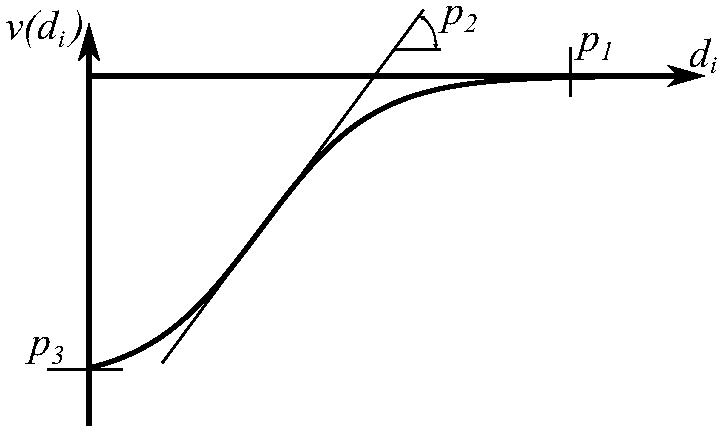
\includegraphics[scale=0.4]{ch3/img/speed_profile.pdf}
	\pgfmathdeclarefunction{speed}{3}{%
		\pgfmathparse{#3 * ( (1)/(1+exp(4*((#1/2)-x)*#2/#3)) - 1 )}%
	}
	\begin{tikzpicture}[>=latex]
		\begin{axis}[
			domain=0:11.5, samples=100,
			enlargelimits=false,
			xmin=0, xmax=12, ymin=-6, ymax=1,
			height=6cm, width=6cm,
			axis lines=middle,
			xlabel=\scriptsize{$d_i$}, ylabel=\scriptsize{$v(d_i)$},
			every axis y label/.style={at=(current axis.above origin),anchor=south },
			every axis x label/.style={at=(current axis.right of origin),anchor=west},
			xtick=\empty, ytick=\empty,
			extra y ticks={-4.7}, extra y tick labels={$p_3$},
			extra x ticks={10}, extra x tick labels={$p_1$}
		]
			\addplot[black,line width=1.5]{speed(7,1,5)};
		\end{axis}
		
		\draw (0.75,1.3) -- ++(240:1) -- ++(60:5) -- ++(240:0.75) -- ++(0.75,0) --++(-0.15,0) coordinate(arco);
		\draw[<->] (arco) arc(0:60:0.6) node [xshift=15] {$p_2$};	
	\end{tikzpicture}
	\caption{Velocity profile}
\end{marginfigure}
from which we obtain a continuous function were the parameters:
\begin{itemize}
\item $p_1$: it is the maximum range, at which considered velocity is zero
\item $p_2$: defines the slope of the curve at ${d_i = p_1/2}$
\item $p_3$: defines the maximum velocity, or the value of the curve for ${d_i = 0}$
\end{itemize}

In figure \ref{fig:obstavoidexample} an example of how the algorithm works is shown. Obviously, signal coming from the algorithm get some sort of filtration to eliminate various source of error.
\begin{figure}[h]
	\centering
	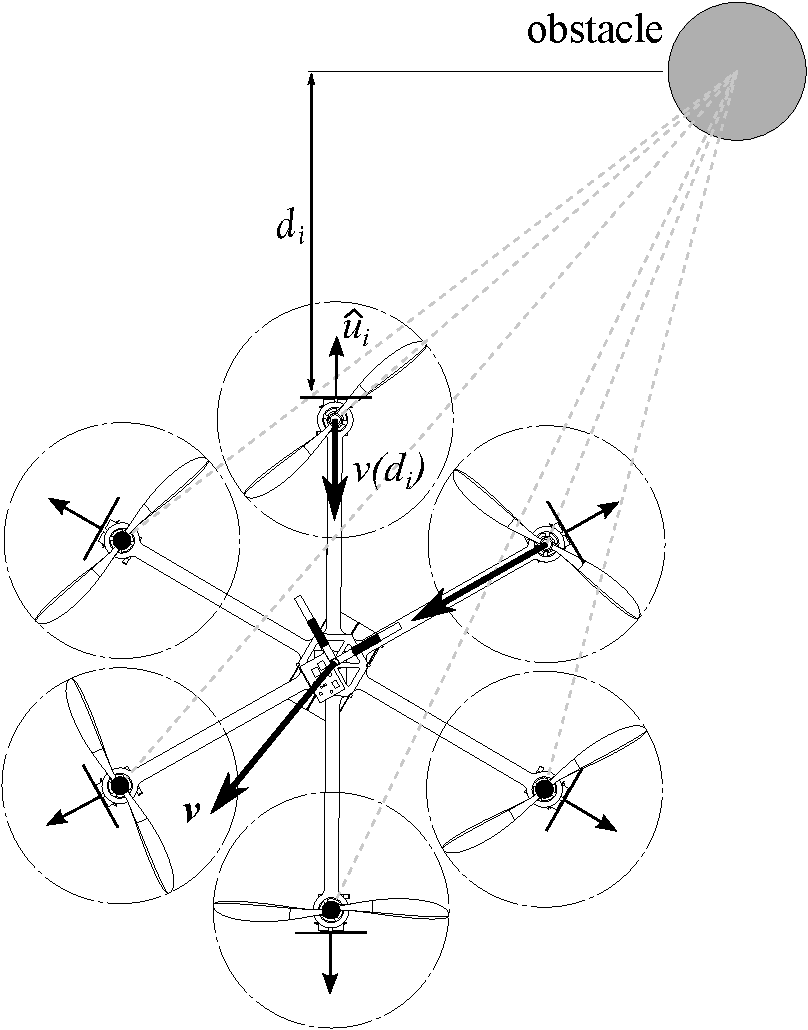
\includegraphics[scale=0.45]{ch3/img/obstavoid_dist.pdf}
	\caption{Example of obstacle avoid algorithm behavior}
	\label{fig:obstavoidexample}
	\forceversofloat
\end{figure}

\myparagraph{Model of range finder}
\begin{figure}[h]
	\centering
	%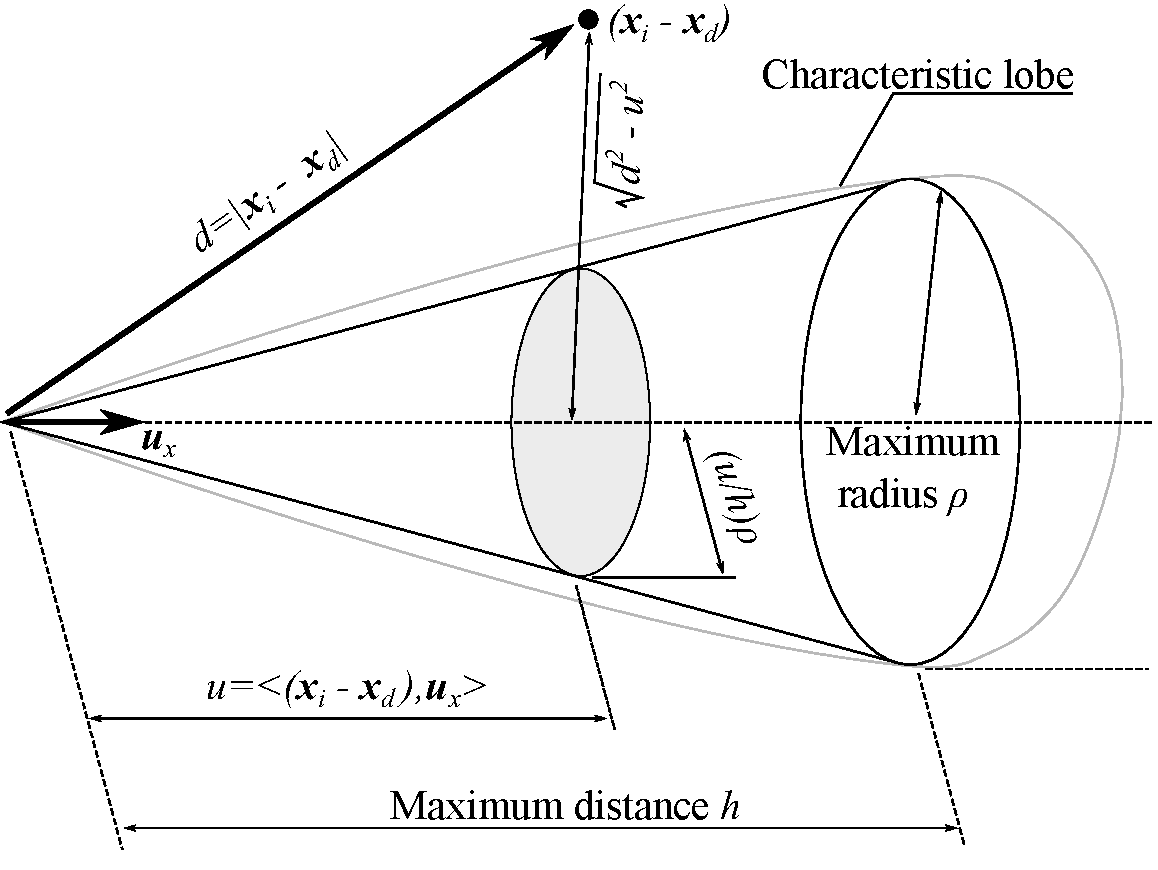
\includegraphics[scale=0.45]{ch3/img/lobe_dimensions.pdf}
	\begin{tikzpicture}[>=latex']
		\draw[dashed,gray] (0,0) .. controls (6cm,3cm) ..  (8.5cm,3.5cm) to[bend left,out=45] (11cm,0cm) to [bend left,in=125] (8.5cm,-3.5cm) .. controls (6cm,-3cm) .. cycle;
	   \draw [fill=gray!40,opacity=40](5cm,0cm) ellipse (0.75cm and 2.05cm);
		\draw (8.5cm,0cm) ellipse (1.25cm and 3.5cm);
		\draw (8.2cm,-3.4cm) -- (0,0) -- (8.2cm,3.4cm);
		\draw[dashed] (0,0) -- (9cm,0);

		\node [circle,inner sep=1pt,fill=black] at (5cm,4cm) {};
		\draw [<->] (5cm,0cm) -- node[pos=0.9,right]{$\sqrt{d_i^2-u^2}$} (5cm,3.9cm);
		\draw [->,line width=1.5] (0cm,0cm) -- (2.5cm,0cm);
		\draw [->,line width=1.5] (0cm,0cm) -- node[above,rotate=38.53]{$d_i = | \mathbf{x}_i^{\Psi} - \mathbf{x}_d|$} (4.9cm,3.9cm);
		\draw [->] (5cm,0cm) -- ++(-70:1.4) node[anchor=west,xshift=3,yshift=-3] {$\dfrac{\rho}{h}u$};
		\node at(4cm,4.3cm) {$(\mathbf{x}_i^{\Psi} - \mathbf{x}_d)$};
		\node at(2.5cm,-0.35cm) {$\hat{\mathbf{u}}_{i}$};

		\draw [->] (8.5cm,0cm) -- ++(-70:2.5) node[anchor=west,xshift=3,yshift=-3] {$\rho$ (maximum radius)};

		\draw (0cm,-0.1cm) -- (0cm,-5cm);
		\draw (4.9cm,-2.2cm) -- (4.9cm,-4cm);
		\draw (8.5cm,-0.1cm) -- (8.5cm,-5cm);
		\draw [<->](0cm,-3.9cm) -- node[pos=0.5,above]{$u=(\mathbf{x}_i^{\Psi} - \mathbf{x}_d) \cdot \hat{\mathbf{u}}_i$} (4.9cm,-3.9cm);
		\draw [<->](0cm,-4.9cm) -- node[pos=0.5,above]{$h$ (maximum range)} (8.5cm,-4.9cm);
		\draw [<-] (9cm,3.5cm) -- ++(45:0.5cm) -- node[pos=0.5,above]{Characteristic lobe} ++(3cm,0); 
	\end{tikzpicture}
	\caption{Range finder algorithm}
\end{figure}
From the simulation point of view the effects of an obstacle are obtained through a model of the characteristic lobe of each range finder. The obstacles are implemented as sets of points, paradigm that brings a little advantage of inserting some noise due to the discontinuities between points, similar to real range finder noise, due to analog to digital conversion.
\begin{equation}
\Psi = \left[ \mathbf{x}_i \,:\,i=1..M  \right]
\end{equation}

For our system we suppose to know exactly the position $\hexastate_d$ and orientation $\rotmat$ of the drone\sidenote{For the obstacle avoidance algorithm only attitude must be know, to project the velocity in ground reference frame}. We define observation versors as follows:
\begin{equation}
\label{eq:versorirangefind}
\left\{ \vers{u}_i \,:\, i=1..6 \right\} \rightarrow \left\{ \vettore{\cos\braces{(i-1)\dfrac{\pi}{3}} \\ -\sin\braces{(i-1)\dfrac{\pi}{3}} \\0} \,:\, i=1..6 \right\}
\end{equation}
The characteristic of the range finder is described with the use of a cone. Distance is evaluated using time of flight of an ultrasonic signal emitted by the oscillator. Mathematically it is possible to define the lobe with a cone in the space, that has axis parallel to the versors defined in \ref{eq:versorirangefind}, and vertex coincident with receiving system. The solid that approximates the characteristic lobe is defined by:
\begin{equation}
\begin{array}{rcl}
x = \dfrac{u}{h} \rho \cos(\theta)
y = \dfrac{u}{h} \rho \sin(\theta)
z = u
\end{array}
\end{equation}
so characteristic lobe is defined by the parameter:
\begin{itemize}
\item $h$: receiver maximum distance
\item $\rho$: receiver maximum lobe dimension
\end{itemize}

\begin{algorithm}[h]
\caption{Range finder points}
\SetKw{KwAs}{as}
\KwData{$h,\,\rho$}
\ForEach{Obstacle \KwAs $\Psi$}{
	\tcc{Exec for each point of an obstacle}
	\For{$i=1$ \KwTo $M$}{ 
		${\mathbf{d}_i^{\Psi} \leftarrow \mathcal{R}^T(\phi,\theta,\psi) \braces{\mathbf{x}_{i,\mathrm{ground}}^{\Psi}-\mathbf{x}_d}}$\;
		\For{$j=0$ \KwTo 5}{
			${D_{i,j}^{\Psi} \leftarrow \mathbf{d}_i^{\Psi} \cdot \vers{u}(j\pi/3)}$\;
			\tcc{Check if the point is in cone, else distance is $\infty$}
			\eIf{$\braces{0\leq D_{i,j}^{\Psi} \leq h}$}{
				\If{$\braces{\mathbf{d}_i^{\Psi} \cdot \mathbf{d}_i^{\Psi} - {D_{i,j}^{\Psi}}^2 \geq \braces{\dfrac{\rho}{h} D_{i,j}^{\Psi}}^2 }$}{
					${D_{i,j}^{\Psi} \leftarrow \infty}$\;
				}
			}{
				${D_{i,j}^{\Psi} \leftarrow \infty}$ \;
			}
		}
	}
}
\tcc{Search minimum distance for each sensor}
$\mathbf{r} \leftarrow [r_j = \infty\,:\,j=0$ \KwTo $5]$\;
\For{$j=0$ \KwTo 5}{
	\ForEach{Obstacle \KwAs $\Psi$}{
		\For{$i=1$ \KwTo $M$}{
			\If{$r_j \geq D_{i,j}^{\Psi}$}{
				$r_j \leftarrow D_{i,j}^{\Psi}$ \;
			}
		}
	}
}
\Return{$\mathbf{r}$}
\end{algorithm}

Given a point ${\mathbf{x}_i \in \Psi}$, if it is inside the cone, the projection of the distance ${\mathbf{x}_d-\mathbf{x}_i}$ on the axis of the cone is the identified distance.

The algorithm describes how each sensor returns the minimum identified distance that is inside its cone. The distances are used to build the velocity vector that avoid the obstacle.

\FloatBarrier